\section[Socio-technical aspects]{Socio-technical aspects\\ \small{(Probably cover this topic in the Discussion and the Conclusion.)}}
\buzzwords{Systems Thinking, Games people play}

\emph{Note: the current thesis doesn't have much on this topic. TBD whether to include it, it's certainly pertinent in my view. Tip: don't use the term Game Theory as I'm not going to establish, test, or evaluate the case studies using an actual theory.}

Many developers fail to address all the issues identified through use of mobile analytics and a key influence is their perceived ability to successfully address issues identified by the analytics. Furthermore, these issues are collectively only one of many demands for their time and attention. Human, organisational, and business factors all influence the extent mobile analytics is a) used and b) the results addressed. This research touches on both the mechanics of applying mobile analytics together with the `game' which are the higher-level human nature aspects which affect the application and the value of applying the mechanics. Figure~\ref{fig:the-mechanics-the-game} provides a simple illustration of the game and the mechanics.

\begin{figure}
    \centering
    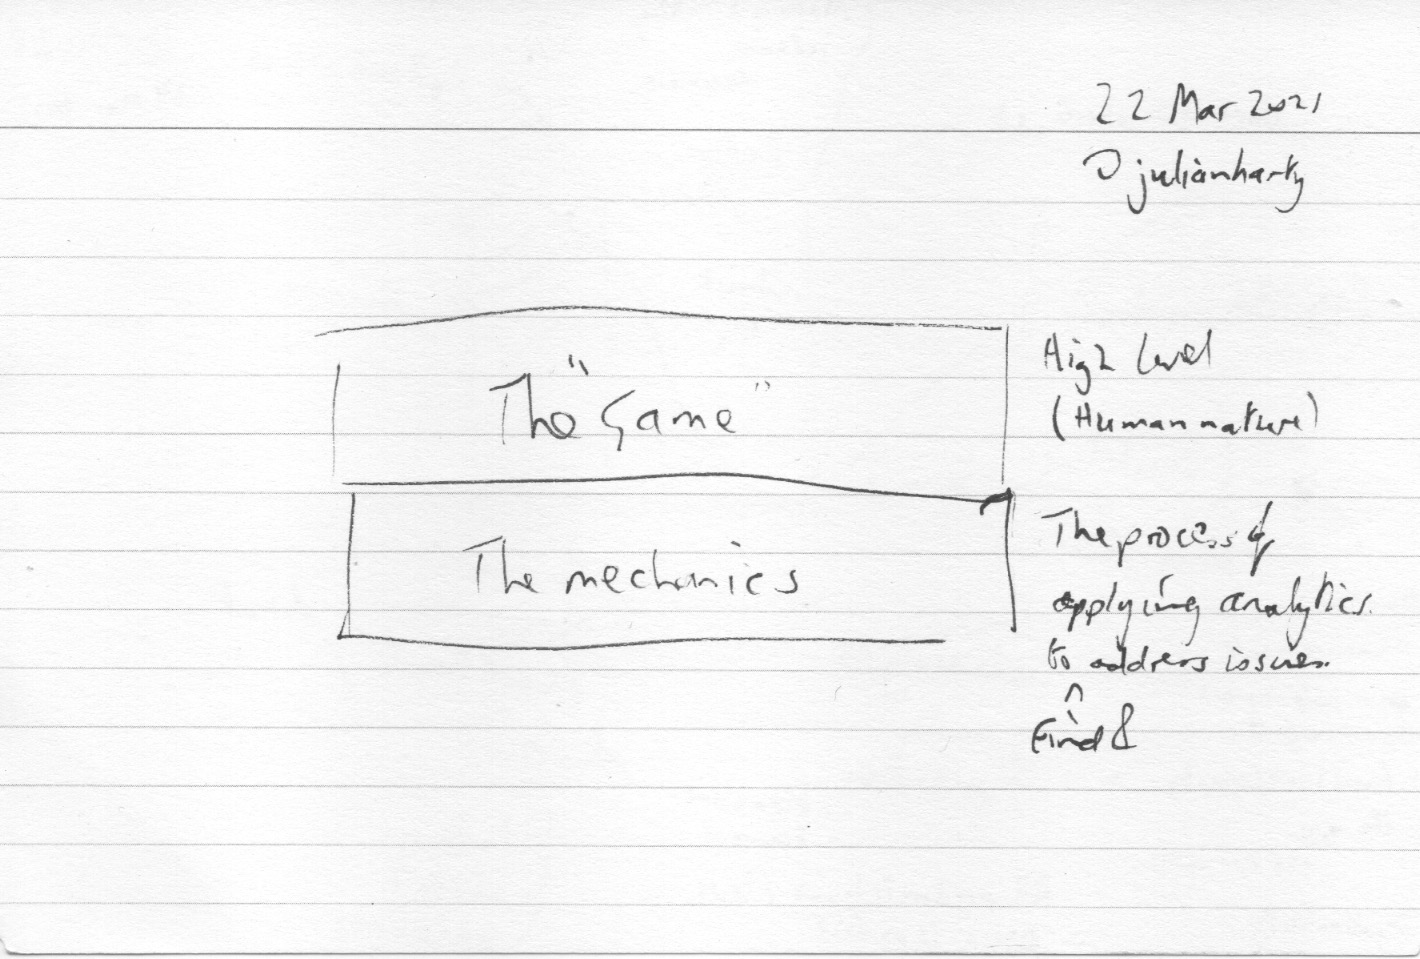
\includegraphics[width=15cm]{images/rough-sketches/The-Mechanics-The-Game.jpeg}
    \caption{The Mechanics and The Game of using Mobile Analytics}
    \label{fig:the-mechanics-the-game}
\end{figure}


\newthought{Living with risks} 
Risks include the risks of not using analytics and the risks of using analytics. Risk taking and risk aversion on the part of the developer, the team, the organisation, the app store organisation, and the end user come to play in the game.

Given the ongoing examples of misdeeds and corruptions in the application of data collected from user's activities and user's content - understanding and analysing the \href{glossary_data_dynamics}{[data] dynamics} of the information gathered, processed, and transferred in support of mobile analytics is also pertinent.

\newthought{Effort and rewards}
Significant data is available for minimal effort; paradoxically the lack of effort may lead to some developers underestimating the usefulness of using this data.

Development teams who choose to invest in analytics are able to reap better and more relevant results. Developers can choose to augment platform-level analytics with in-app analytics to augment or supersede aspects of what the platform provides.

\newthought{Risks and choices}
Developers can choose when they will pay attention to the analytics; they can also choose the extent they wish to integrate analytics into their apps. 

There are risks and responsibilities of the effects of collecting data and performing analysis on that data, practices outstrip legislation. It remains possible for sensitive findings to be discovered through the use of mobile analytics, nonetheless the ethical challenges are not unique to mobile analytics~\footnote{Arosha mentioned \href{https://www.orbit-rri.org/}{ORBIT-RRI} and their ~\href{https://www.journals.elsevier.com/journal-of-responsible-technology}{Journal of Responsible Technology}. There are various areas that overlap and potentially align in their concepts, I've not found much relevant concrete material yet, this footnote is a reminder (it is not intended to be part of my thesis.}.

\newthought{Freedom and responsibility}~\label{newthought-freedom-and-responsibility}
Developers often have more freedom in relation to how an app behaves than the users of their apps do. In practice the vast majority of Android apps in Google Play use and collect mobile analytics, the only material choice the users have is whether to use or not use a particular app. Sometimes the freedom is to \emph{not make a decision} (as mentioned earlier). Making a decision may have consequences. Not making a decision may have consequences. 

Who gets to choose may also be influenced by the larger organisation developers belong to. For example, in some large enterprises developers of an individual app may have to use prescribed mobile analytics rather than being able to make an independent [informed] choice.


\newthought{Minimise harm maximise value address material known issues}~\label{newthought-do-no-net-harm}
In the field of doctors there are discussions by \citealt{Schuenemann2011_guidelines2_0_do_no_net_harm} and \citealt{Sokolf6426_2013_first_do_no_harm_revisited} on \emph{do no net harm}. This has been eloquently adapted to \emph{``A competent and caring physician is one who never causes unintentional or unnecessary harm.", Stephen Ross Workman, MD}~\url{https://www.bmj.com/content/347/bmj.f6426/rr/671112}. Implicitly it could also apply to what users expect from the mobile apps they install and use. So, perhaps a the concept could be extended to the following maxim?: \emph{an app developer not only never causes unintentional or unnecessary harm, they also strive to address whatever harms do affect the users of their apps while also satisfying for other demands}~\footnote{In medicine there have been similar discussions on freedom and responsibility, and in particular on aftercare of what they publish~\citep{rennie1998_freedom_and_responsibility_in_medical_publication}.}.

MUST-DO expand on~\citep{shklovski2014_leakiness_and_creepiness_in_app_space_perceptions_of_privacy_and_mobile_app_use, zhou2017_user_perceived_control_trust_etc_smartphone}.

\textbf{MUST-DO} Explore these themes in the Discussion chapter. Consider separating: 1) those supported by primary evidence in the case studies (a subset of the experiences from the field, some evidence is protected by confidentiality agreements, etc.), 2) those more speculative in nature/based on literature and hence topics for further research.

\isabel{Ask Fiona Charles about her ethics for software engineers}

\section{Snippets to consider in this topic}

\begin{itemize}
    \item The integration of analytics with code owners to alert developers (code owners) when issues are detected that exceed a threashold. \url{https://docs.sentry.io/product/issues/issue-owners/} and see \url{https://docs.github.com/en/repositories/managing-your-repositorys-settings-and-features/customizing-your-repository/about-code-owners} (I believe there are similar features available in GitLab)
\end{itemize}